\documentclass{article}
\usepackage[accepted]{icml2025}
\usepackage{microtype}
\usepackage{booktabs}
\usepackage{amsmath,amssymb,amsthm,bm}
\usepackage{mathtools}
\usepackage{graphicx}
\usepackage{hyperref}
\usepackage[capitalize,noabbrev]{cleveref}
\usepackage{xcolor}
\usepackage{tikz}
\usetikzlibrary{arrows.meta,positioning,fit,backgrounds,calc}

\graphicspath{{../figures/}}

% ---- Math shortcuts ----
\DeclarePairedDelimiter{\norm}{\lVert}{\rVert}
\DeclareMathOperator*{\argmin}{arg\,min}
\DeclareMathOperator{\rank}{rank}
\DeclareMathOperator{\spark}{spark}
\DeclareMathOperator{\supp}{supp}
\DeclareMathOperator{\STFT}{STFT}
\DeclareMathOperator{\sgn}{sgn}
\DeclareMathOperator{\soft}{soft}
\DeclareMathOperator{\SVT}{SVT}
\newcommand{\R}{\mathbb{R}}
\newcommand{\D}{\bm{D}}
\newcommand{\M}{\bm{M}}
\newcommand{\Y}{\bm{Y}}
\newcommand{\X}{\bm{X}}
\newcommand{\Ev}{\bm{E}}
\newcommand{\A}{\bm{A}}
\newcommand{\Hb}{\bm{H}}
\newcommand{\xv}{\bm{x}}
\newcommand{\yv}{\bm{y}}
\newcommand{\av}{\bm{\alpha}}

% ---- Ablation numbers (from experiments/results/ablation_*.csv) ----
\newcommand{\ABLnmfA}{$2.2$} \newcommand{\ABLnmfB}{$1.9$}
\newcommand{\ABLnmfC}{$1.8$} \newcommand{\ABLnmfD}{$1.5$}
\newcommand{\ABLksvdA}{$1.4$} \newcommand{\ABLksvdB}{$2.3$}
\newcommand{\ABLksvdC}{$\mathbf{2.7}$} \newcommand{\ABLksvdD}{$2.7$}
\newcommand{\ABLrpcaA}{$-3.9$} \newcommand{\ABLrpcaB}{$-3.6$}
\newcommand{\ABLrpcaC}{$-3.2$} \newcommand{\ABLrpcaD}{$\mathbf{-2.3}$}

\icmltitlerunning{Unmixing the Music}

\begin{document}

\twocolumn[
\icmltitle{Unmixing the Music: Sparse, Low-Rank, and Deep\\
Compressed-Sensing Approaches to Music Source Separation}

\icmlsetsymbol{equal}{*}
\begin{icmlauthorlist}
\icmlauthor{Taka Khoo}{dart}
\end{icmlauthorlist}
\icmlaffiliation{dart}{Thayer School of Engineering, Dartmouth College, Hanover, NH, USA}
\icmlcorrespondingauthor{Taka Khoo}{taka.khoo.th@dartmouth.edu}
\icmlkeywords{source separation, sparse coding, dictionary learning, robust PCA, algorithm unrolling}
\vskip 0.3in
]
\printAffiliationsAndNotice{}

\begin{abstract}
Music source separation, recovering vocals and accompaniment from a single
mixture, is approached either by classical signal-processing decompositions or by
large end-to-end networks. We show that a wide span of these methods are one idea:
recovery of a structured (sparse or low-rank) representation of the time-frequency
spectrogram. On a shared short-time Fourier front end we build four separators,
Robust PCA, supervised non-negative matrix factorization, K-SVD with
sparse-representation classification, and a deep sparse coding network that unrolls
a non-negative proximal solver and learns its dictionaries end-to-end, and place
them on a single structure-recovery spectrum. On 25 held-out MUSDB18 tracks the
methods order cleanly: training-free baselines trail supervised dictionaries, and
the unrolled deep coder is the strongest non-oracle separator on both sources
(vocal SI-SDR $2.0$ dB, accompaniment $8.3$ dB) while being the fastest learned
model. We pair every method with the recovery condition that governs it and report
a negative result: the learned dictionaries are highly coherent ($\mu\approx0.85$),
so worst-case guarantees are vacuous at the operating sparsity, yet separation
succeeds. Code, models, and audio are released.
\end{abstract}

\section{Introduction}
\label{sec:intro}
Single-channel music source separation recovers the constituent stems of a
recording given only the final mixture. It is hard because mixing destroys
information: many stem configurations explain the same
mixture~\cite{cano2019introduction}. Progress has come from two largely separate
traditions. The first is model-based: non-negative matrix factorization
(NMF)~\cite{lee1999nmf,smaragdis2007convolutive}, low-rank-plus-sparse
decompositions~\cite{huang2012rpca}, and dictionary
learning~\cite{aharon2006ksvd} impose explicit structural priors. The second is
data-driven: deep networks trained end-to-end~\cite{stoter2019openunmix,%
defossez2021demucs,rouard2023htdemucs} define the current state of the art.

\begin{figure}[t]
\centering
\resizebox{\linewidth}{!}{%
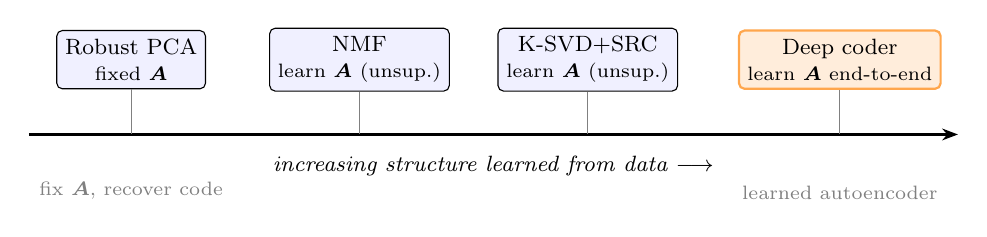
\begin{tikzpicture}[font=\footnotesize,
  m/.style={draw,rounded corners=2pt,align=center,minimum height=7mm,
            fill=blue!6,line width=0.4pt,inner sep=3pt},
  ours/.style={m,fill=orange!14,draw=orange!70,line width=0.8pt}]
\draw[-{Stealth[length=2mm]},line width=0.8pt] (-0.2,0)--(11.6,0);
\node[anchor=north] at (5.7,-0.15)
  {\itshape increasing structure learned from data $\longrightarrow$};
\node[m] (a) at (1.1,0.95) {Robust PCA\\\scriptsize fixed $\A$};
\node[m] (b) at (4.0,0.95) {NMF\\\scriptsize learn $\A$ (unsup.)};
\node[m] (c) at (6.9,0.95) {K-SVD$+$SRC\\\scriptsize learn $\A$ (unsup.)};
\node[ours] (d) at (10.1,0.95) {Deep coder\\\scriptsize learn $\A$ end-to-end};
\foreach \n in {a,b,c,d}{\draw[gray,line width=0.3pt] (\n.south)--(\n.south|-0,0);}
\node[anchor=south,gray] at (1.1,-0.95) {\scriptsize fix $\A$, recover code};
\node[anchor=south,gray] at (10.1,-0.95) {\scriptsize learned autoencoder};
\end{tikzpicture}}
\caption{The four separators as points on one structure-recovery spectrum. All
solve the same underdetermined system $\yv=\A\xv$ with a sparse code; they differ
only in how much of the dictionary $\A$ is learned, from a fixed convex split to a
fully trained unrolled solver.}
\label{fig:spectrum}
\end{figure}

\paragraph{The unifying view.}
These traditions are two ends of a single axis (\cref{fig:spectrum}). The
magnitude spectrogram of a voiced frame is sparse (a few formant atoms) and the
sustained accompaniment is low-rank. These are not separate assumptions but two
sides of the same coin: the rank of a matrix is the $\ell_0$ norm of its singular
spectrum and the nuclear norm is the corresponding $\ell_1$ relaxation, so ``few
active atoms'' and ``few active singular vectors'' are the same prior applied to a
vector and to a matrix~\cite{candes2011rpca}. The recovery problem is in every
case the underdetermined system $\yv=\A\xv$ with a sparse code: the classical half
of the subject fixes the dictionary $\A$ and recovers the code, while dictionary
learning, K-SVD, and NMF instead \emph{learn} $\A$ from data. Deep masking networks
sit at the learned end of this same continuum: a sparse coding network is, in a
precise sense, a learned autoencoder~\cite{gregor2010lista,papyan2017cnncsc}, an
unrolled sparse-recovery solver whose operators are trained by
backpropagation~\cite{monga2021unrolling}.

\paragraph{Contributions.} (i) We cast vocal/accompaniment separation as
structured recovery and instantiate four separators that share a short-time
Fourier transform (STFT) front end and one evaluation harness. (ii) We build a deep
sparse coding network that predicts a soft mask by unrolling a non-negative
proximal-gradient iteration and learning its dictionaries end-to-end, and show it
is the strongest non-oracle separator while being the fastest learned model. (iii)
We pair each method with its recovery condition and report a negative result on
dictionary coherence. Code, weights, and audio are released.

\paragraph{Related work.}
NMF for audio dates to \citet{smaragdis2003nmf}; supervised and convolutive
variants~\cite{smaragdis2007convolutive,fevotte2009isnmf} pre-train one dictionary
per source. Robust-PCA singing-voice separation~\cite{huang2012rpca} and
REPET~\cite{rafii2013repet} exploit the repetitive, low-rank structure of
accompaniment. K-SVD~\cite{aharon2006ksvd} learns overcomplete sparsifying
dictionaries and SRC~\cite{wright2009src} classifies by reconstruction residual.
On the deep side, Spleeter, Open-Unmix, and Demucs train end-to-end
masks~\cite{stoter2019openunmix,defossez2021demucs,rouard2023htdemucs}, while a
complementary line reads such networks as unrolled sparse coding: LISTA unrolls
ISTA~\cite{gregor2010lista}, CNNs admit a convolutional-sparse-coding
reading~\cite{papyan2017cnncsc}, and supervised deep sparse coding networks have
been studied for image classification~\cite{sun2019scn}. Our learned separator
instantiates this unrolling idea for music spectrogram masking.

\section{Background: Spectrograms, Stems, and Masking}
\label{sec:background}
The short-time Fourier transform slides a window across $y(t)$ and takes a DFT in
each window, producing a complex matrix $\Y\in\mathbb C^{F\times T}$ with $F$
frequency bins and $T$ frames. Its modulus $\M=\lvert\Y\rvert$ is a nonnegative
image (brightness is energy) and its argument $\angle\Y$ is the phase; the transform
is invertible. A finished song is a sum of source \emph{stems}, and because the STFT
is linear the mixture spectrogram is approximately the sum of the source
spectrograms. Rather than predict a source spectrogram outright, we predict a
\emph{mask} $\M_c\in[0,1]^{F\times T}$ that scales each cell and resynthesize with
the mixture phase. The minimum-mean-square-error mask under locally uncorrelated
Gaussian sources is the ideal ratio mask
$\M_c^{\mathrm{IRM}}=\lvert\Y_c\rvert^2/\sum_k\lvert\Y_k\rvert^2$; it needs the true
sources and so serves only as an oracle ceiling. Two empirical regularities make the
masks recoverable (\cref{fig:triptych}): a voiced frame places energy on a sparse
set of harmonics, and sustained accompaniment reuses a few spectral templates and is
therefore low-rank, the two structures compressed sensing is built to exploit.

\begin{figure}[t]
\centering
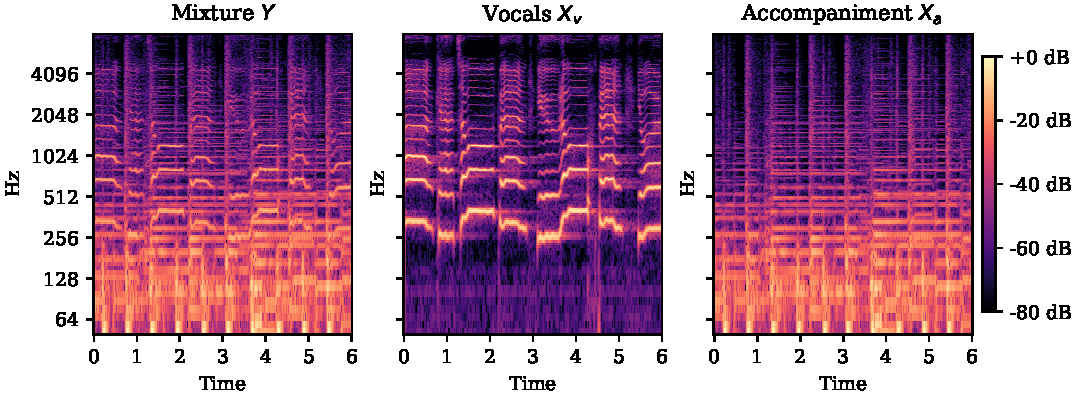
\includegraphics[width=\linewidth]{fig_triptych.pdf}
\caption{Log-magnitude STFT of a test clip: the mixture, the true vocals (a sparse
harmonic scaffold), and the true accompaniment (denser and lower-rank). Our methods
reverse the sum.}
\label{fig:triptych}
\end{figure}

\section{Preliminaries}
\label{sec:theory}
Write $\norm{\xv}_0=\lvert\supp(\xv)\rvert$. Given $\A\in\R^{m\times N}$ with
$m\ll N$ and $\yv=\A\xv$ for an $s$-sparse $\xv$, the combinatorial program
$\min\norm{\bm z}_0$ s.t. $\A\bm z=\yv$ is NP-hard; its $\ell_1$ relaxation is a
linear program. Three sufficient conditions certify exactness: $\spark(\A)>2s$
(uniqueness); the restricted isometry property
$(1-\delta_s)\norm{\xv}_2^2\le\norm{\A\xv}_2^2\le(1+\delta_s)\norm{\xv}_2^2$ with
$\delta_{2s}<\sqrt2-1$~\cite{candes2006rip}; and the verifiable coherence bound
\begin{equation}
\label{eq:coh}
s<\tfrac12\!\left(1+\tfrac1{\mu(\A)}\right),\qquad
\mu(\A)=\max_{i\ne j}\lvert\langle\A_i,\A_j\rangle\rvert,
\end{equation}
under which orthogonal matching pursuit (OMP) and $\ell_1$ minimization recover
every $s$-sparse signal~\cite{tropp2007omp,donoho2006cs}. For low rank, the nuclear
norm $\norm{\X}_*=\sum_i\sigma_i(\X)$ is the convex surrogate, and Robust PCA splits
$\M=\X+\Ev$ into low-rank $\X$ and sparse $\Ev$ by principal component
pursuit~\cite{candes2011rpca}.

\section{Method}
\label{sec:method}
\paragraph{Front end.} For a mono mixture $y(t)$, the STFT is
$\Y\in\mathbb C^{F\times T}$ with magnitude $\M=\lvert\Y\rvert$ and phase
$\angle\Y$. Every separator emits a soft mask $\M_c\in[0,1]^{F\times T}$ and
resynthesizes $\hat y_c=\STFT^{-1}(\M_c\odot\Y)$ with the mixture phase; given
nonnegative magnitude estimates $\widehat\M_c$ we use Wiener masks
$\M_c=\widehat\M_c^{2}/\sum_k\widehat\M_k^{2}$. The methods differ only in how they
estimate $\widehat\M_c$ (\cref{tab:taxonomy}).

\begin{table}[t]
\caption{The four separators as one family: a structural prior, its penalty, and a
learning mode.}
\label{tab:taxonomy}
\centering
\footnotesize
\setlength{\tabcolsep}{4pt}
\begin{tabular}{@{}llll@{}}
\toprule
\textbf{Method} & \textbf{Prior} & \textbf{Penalty} & \textbf{Learning} \\
\midrule
RPCA      & low-rank$+$sparse & nuclear$+\ell_1$ & none \\
NMF       & nonneg.\ parts    & KL div.\         & unsup. \\
K-SVD     & sparse code       & $\ell_0\!\le\!s$ & unsup. \\
SCN       & unrolled sparse   & elastic-net      & end-to-end \\
\bottomrule
\end{tabular}
\end{table}

\paragraph{(A) Robust PCA.} We solve $\min_{\X,\Ev}\norm{\X}_*+\lambda\norm{\Ev}_1$
s.t. $\X+\Ev=\M$, $\lambda=1/\sqrt{\max(F,T)}$, by inexact ALM (singular-value
thresholding for the nuclear prox, soft-thresholding for $\ell_1$). The low-rank
$\X$ is the accompaniment and the sparse $\Ev$ the vocal proxy, the same intuition
that pulls a moving foreground out of a static background in surveillance video.
Training-free.

\paragraph{(B) Supervised NMF.} We pre-train one nonnegative dictionary per source,
$\M_c\approx\D_c\Hb_c$, by Lee-Seung KL multiplicative
updates~\cite{lee2000algorithms}, which are a majorization-minimization scheme that
cannot increase the loss. At test time we fix $\D=[\D_v\mid\D_a]$ and solve for the
activations, then split $\widehat\M_v=\D_v\Hb_v$ and $\widehat\M_a=\D_a\Hb_a$.

\paragraph{(C) K-SVD + SRC.} We learn an overcomplete dictionary per source by
K-SVD~\cite{aharon2006ksvd} (alternating OMP coding with rank-one atom updates that
are Eckart-Young optimal), sparse-code each mixture frame on $[\D_v\mid\D_a]$, and
route energy by the SRC residual rule
$c^\star=\argmin_c\norm{\yv-\D_c\av_c}_2$~\cite{wright2009src}. Coherence
\cref{eq:coh} governs when this per-frame code is unique.

\paragraph{(D) Deep sparse coding network.}
Our learned separator predicts the mask by unrolling a non-negative sparse solver
and learning its dictionaries end-to-end. Each composite module is an
expand-then-reduce hourglass (\cref{fig:cmod}): a fat dictionary lifts the frame to
an over-complete code, a tall dictionary compresses it, each computed as
\begin{equation}
\av^{(\ell)}=\argmin_{\av\ge0}\tfrac12\norm{\bm u-\D^{(\ell)}\av}_2^2
+\lambda_1\norm{\av}_1+\tfrac{\lambda_2}2\norm{\av}_2^2,
\end{equation}
solved by $K$ steps of non-negative FISTA, each a matrix multiply, gradient step,
and clamp $\av_k=[\bm z_k-\tfrac1L\D^\top(\D\bm z_k-\bm u)-\tfrac{\lambda_1}L]_+$
with Nesterov momentum. All operations are differentiable, so the dictionaries
$\D^{(\ell)}$ and shrinkages $\lambda_1,\lambda_2$ train by backpropagation against
the ideal ratio mask with an $\ell_1$ penalty on the codes. This is the LISTA
construction~\cite{gregor2010lista} specialized to non-negative codes and a masking
output; the clamp is a proximal step, and run to convergence the iteration attains
the optimal $O(1/k^2)$ rate~\cite{beck2009fista}. We stack four modules with a
$\pm2$-frame temporal context window ($1.44$M parameters). A simultaneous-OMP
variant gives a stereo joint-sparsity extension~\cite{tropp2006somp}.

\begin{figure}[t]
\centering
\resizebox{0.92\linewidth}{!}{%
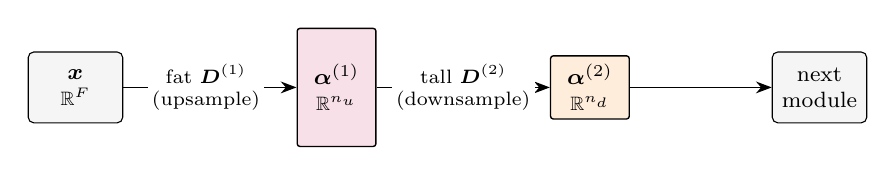
\begin{tikzpicture}[font=\footnotesize,
  io/.style={draw,rounded corners=2pt,align=center,minimum height=9mm,
             minimum width=12mm,fill=gray!8,line width=0.4pt,inner sep=3pt},
  tallb/.style={draw,rounded corners=1pt,align=center,minimum width=10mm,
                minimum height=15mm,fill=purple!12,line width=0.5pt,inner sep=3pt},
  shortb/.style={draw,rounded corners=1pt,align=center,minimum width=10mm,
                 minimum height=8mm,fill=orange!14,line width=0.5pt,inner sep=3pt},
  lbl/.style={fill=white,inner sep=1.5pt,font=\scriptsize,align=center},
  arr/.style={-{Stealth[length=2mm]},line width=0.5pt}]
\node[io] (x) {$\xv$\\\scriptsize$\R^F$};
\node[tallb,right=22mm of x] (a1) {$\av^{(1)}$\\\scriptsize$\R^{n_u}$};
\node[shortb,right=22mm of a1] (a2) {$\av^{(2)}$\\\scriptsize$\R^{n_d}$};
\node[io,right=18mm of a2] (out) {next\\module};
\draw[arr] (x)--(a1); \node[lbl] at ($(x)!0.5!(a1)$){fat $\D^{(1)}$\\(upsample)};
\draw[arr] (a1)--(a2); \node[lbl] at ($(a1)!0.5!(a2)$){tall $\D^{(2)}$\\(downsample)};
\draw[arr] (a2)--(out);
\end{tikzpicture}}
\caption{One composite module: a fat dictionary lifts the frame to an over-complete
sparse code, a tall dictionary compresses it. The expand-then-reduce shape is the
autoencoder hourglass with a sparse bottleneck.}
\label{fig:cmod}
\end{figure}

\section{Experiments}
\label{sec:exp}
\paragraph{Setup.} We use the MUSDB18 benchmark~\cite{rafii2017musdb18}, separating
vocals from accompaniment. Dictionaries and the deep model are trained on the train
split; all numbers are medians over $25$ held-out test tracks at $22.05$ kHz,
$2048$-point STFT, hop $512$. We report scale-invariant SDR~\cite{leroux2019sdr} and
compare against two training-free baselines, median-filtering HPSS and
REPET-SIM~\cite{fitzgerald2010hpss,rafii2013repet}; two trivial floors (returning
the mixture; a random mask); and the ideal ratio/binary mask oracles. NMF uses
$K{=}64$ KL atoms, K-SVD $K{=}96$, $s{=}10$, and the deep coder four modules,
$1.44$M parameters, trained on a laptop GPU.

\begin{table}[t]
\caption{Median SI-SDR (dB) on $25$ MUSDB18 test tracks with mean inference time per
$6$\,s clip. Best non-oracle in \textbf{bold}.}
\label{tab:main}
\centering
\small
\begin{tabular}{@{}lccc@{}}
\toprule
\textbf{Method} & \textbf{Vocals} & \textbf{Accomp.} & \textbf{Time (s)} \\
\midrule
Mixture (no split) & $-3.7$ & $4.0$ & $0.00$ \\
Random mask        & $-3.9$ & $2.9$ & $0.01$ \\
HPSS (median)      & $-11.9$& $-1.4$& $0.25$ \\
REPET-SIM          & $-0.7$ & $2.9$ & $0.08$ \\
\midrule
RPCA               & $-3.1$ & $0.2$ & $1.14$ \\
NMF (supervised)   & $0.5$  & $5.1$ & $0.46$ \\
K-SVD + SRC        & $0.8$  & $7.1$ & $0.28$ \\
SCN (ours)         & $\mathbf{2.0}$ & $\mathbf{8.3}$ & $\mathbf{0.12}$ \\
\midrule
Oracle IRM / IBM   & $10.2$ & $15.8$ & --- \\
\bottomrule
\end{tabular}
\end{table}

\paragraph{Main result.}
\Cref{tab:main} and \cref{fig:bars} show a clean ordering. The floors calibrate the
scale: returning the mixture already scores $+4.0$ dB on accompaniment because the
band dominates the energy, so accompaniment numbers read against this floor. The
training-free baselines are weak (HPSS falls below even the mixture floor). The
supervised dictionary methods improve sharply, and the deep sparse coding network is
the best non-oracle separator on both sources ($2.0$ dB vocals, $8.3$ dB
accompaniment), beating the best classical method by $\approx1.2$ dB on each, while
being the fastest learned model since its forward pass is a fixed number of matrix
multiplies rather than an iterative solve. Soft (ratio) masks beat hard binary masks
by $\approx1$ dB for every method. All methods stay below the oracle ceilings, as
any mixture-phase magnitude mask must.

\begin{figure}[t]
\centering
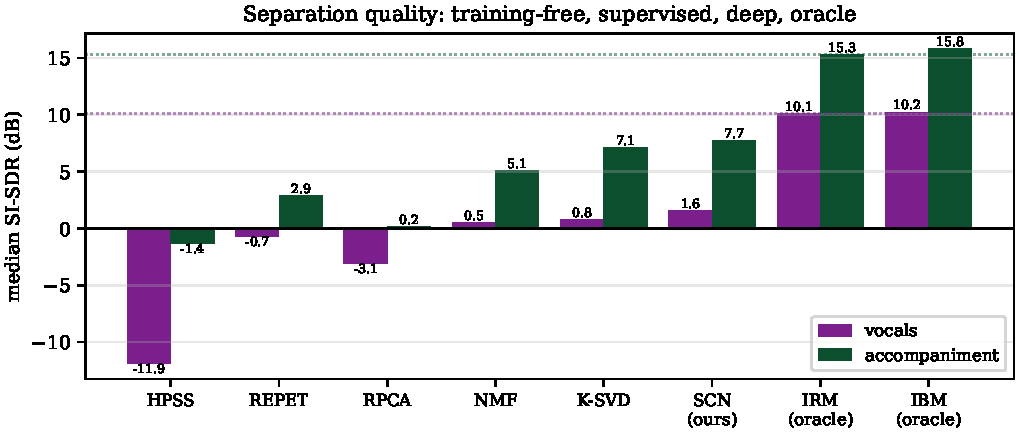
\includegraphics[width=0.9\linewidth]{fig_results_bars.pdf}
\caption{Median SI-SDR by method; dotted lines mark the oracle ceilings. Supervision
and unrolled learning each add a clear increment over the training-free baselines.}
\label{fig:bars}
\end{figure}

\paragraph{Per-track spread, masks, stereo, cost.}
Medians hide variance, so \cref{fig:box} plots the per-track vocal SI-SDR
distribution: the deep model shifts the whole distribution rightward, not only the
easy tracks, though every method has a long lower tail on dense, vocal-quiet
mixtures. The masking strategy matters independently of the model: soft (ratio)
masks beat hard binary masks by $\approx1$ dB for every method ($2.1$ vs $1.0$ dB
for the deep coder), because a continuous gain keeps the partial-overlap cells a
binary decision discards. The stereo simultaneous-OMP separator
(\cref{sec:method}) reaches $0.9$/$7.3$ dB on $10$ stereo tracks, matching the mono
dictionary it is built on while keeping the two channels consistent.
\Cref{tab:cost} contrasts model size and per-clip cost: the deep coder is the
smallest learned model we train and the fastest at test time, an order of magnitude
quicker than the iterative RPCA solve, because its forward pass is a fixed number of
matrix multiplies.

\begin{figure}[t]
\centering
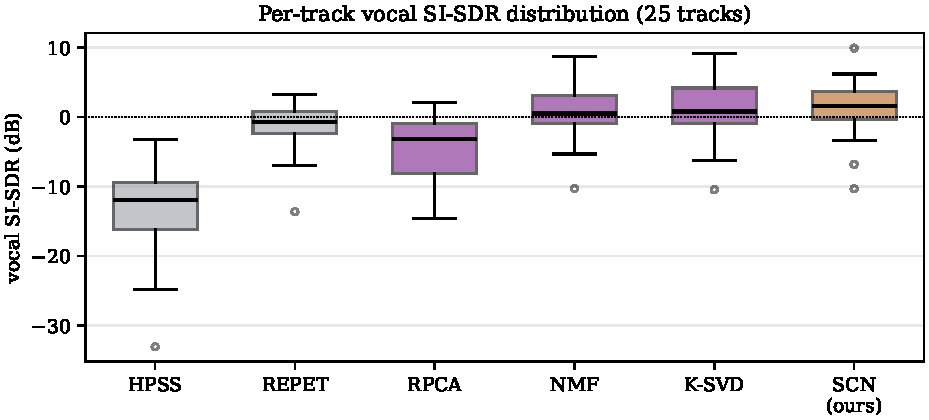
\includegraphics[width=0.92\linewidth]{fig_boxplot.pdf}
\caption{Per-track vocal SI-SDR over the $25$ test tracks. The deep model shifts the
full distribution rather than only improving easy tracks.}
\label{fig:box}
\end{figure}

\begin{table}[t]
\caption{Model size and per-clip cost. Classical methods store fixed dictionaries;
SCN learns dictionaries and shrinkages end-to-end.}
\label{tab:cost}
\centering
\footnotesize
\setlength{\tabcolsep}{5pt}
\begin{tabular}{@{}lccc@{}}
\toprule
\textbf{Method} & \textbf{Trains?} & \textbf{Params} & \textbf{Test (s)} \\
\midrule
RPCA       & no          & ---     & $1.14$ \\
NMF        & dict.\ only & $0.13$M & $0.46$ \\
K-SVD      & dict.\ only & $0.20$M & $0.28$ \\
SCN (ours) & end-to-end  & $1.44$M & $0.12$ \\
\bottomrule
\end{tabular}
\end{table}

\paragraph{Ablations.}
\Cref{tab:abl} sweeps the central knobs. Supervised NMF is \emph{best at the
smallest} dictionary ($K{=}16$): with limited data a small dictionary is a stronger
prior, a regularization effect. K-SVD improves with the sparsity budget to $s{=}10$
then saturates. RPCA improves as the penalty $\lambda$ grows, pushing more energy
into the low-rank band and leaving a cleaner sparse vocal, so the canonical $\lambda$
is conservative for this task. The learned dictionaries themselves are musically
sensible: \cref{fig:atoms} shows the NMF vocal atoms concentrating harmonic ridges
in the formant region while the accompaniment atoms spread lower and wider, the
parts-based structure NMF is designed to recover. The Robust PCA solver is
well-behaved too: \cref{fig:conv} shows its residual reaching $10^{-7}$ in $38$
iterations and the mixture's singular spectrum collapsing after a handful of
components, the empirical evidence for the low-rank accompaniment prior.

\begin{figure}[t]
\centering
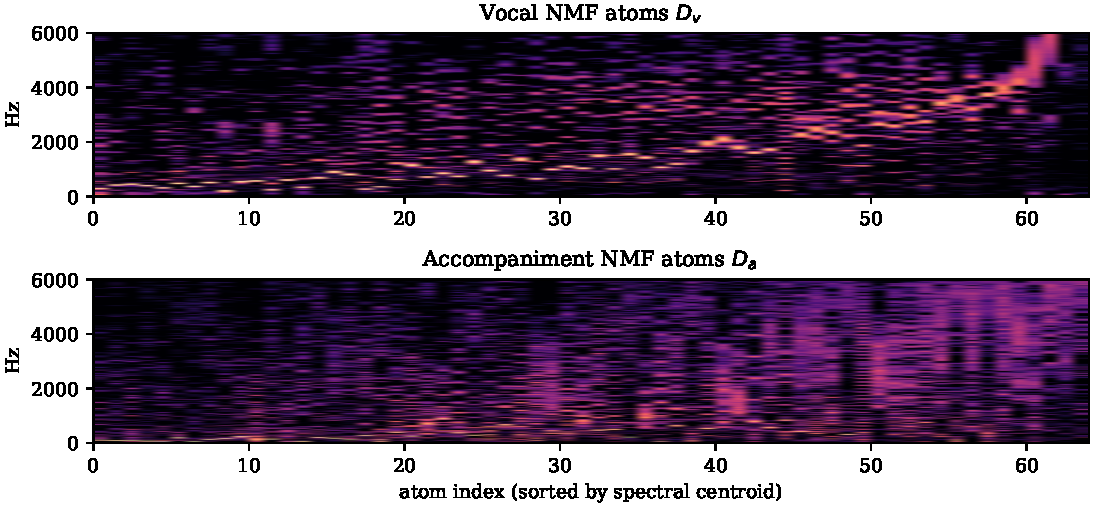
\includegraphics[width=\linewidth]{fig_nmf_atoms.pdf}
\caption{Supervised NMF dictionaries, atoms sorted by spectral centroid: vocal atoms
(top) ride the formant region, accompaniment atoms (bottom) spread lower.}
\label{fig:atoms}
\end{figure}

\begin{figure}[t]
\centering
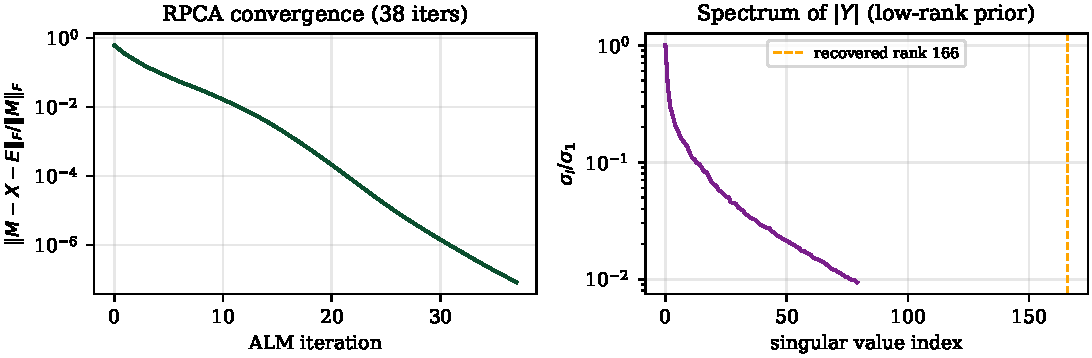
\includegraphics[width=\linewidth]{fig_rpca_converge.pdf}
\caption{Left: relative residual of the principal-component-pursuit iteration.
Right: normalized singular spectrum of the mixture magnitude, justifying the
low-rank accompaniment prior.}
\label{fig:conv}
\end{figure}

\begin{table}[t]
\caption{Ablations (median vocal SI-SDR, dB, $12$ tracks).}
\label{tab:abl}
\centering
\footnotesize
\setlength{\tabcolsep}{4.5pt}
\begin{tabular}{@{}lcccc@{}}
\toprule
NMF atoms $K$        & $16$ & $32$ & $64$ & $128$ \\
Vocal SI-SDR         & \ABLnmfA & \ABLnmfB & \ABLnmfC & \ABLnmfD \\
\midrule
K-SVD sparsity $s$   & $3$ & $5$ & $10$ & $15$ \\
Vocal SI-SDR         & \ABLksvdA & \ABLksvdB & \ABLksvdC & \ABLksvdD \\
\midrule
RPCA $\lambda$ scale & $0.5$ & $1.0$ & $1.5$ & $2.0$ \\
Vocal SI-SDR         & \ABLrpcaA & \ABLrpcaB & \ABLrpcaC & \ABLrpcaD \\
\bottomrule
\end{tabular}
\end{table}

\begin{figure}[t]
\centering
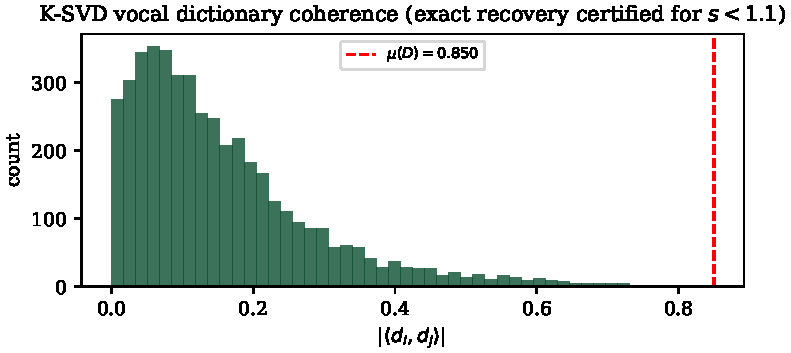
\includegraphics[width=0.78\linewidth]{fig_ksvd_coherence.pdf}
\caption{Off-diagonal coherence of the learned K-SVD vocal dictionary. The
worst-case bound certifies recovery only for $s\!\lesssim\!1$, but separation at
$s{=}10$ works, evidence of an average-case-versus-worst-case gap.}
\label{fig:coh}
\end{figure}

\paragraph{Coherence: a negative result.}
The recovery condition \cref{eq:coh} needs low coherence, but a dictionary trained
for reconstruction is coherent. \Cref{fig:coh} shows the learned K-SVD vocal
dictionary has $\mu\approx0.85$, so \cref{eq:coh} certifies exact recovery only for
$s<\tfrac12(1+1/\mu)\approx1.1$, far below the $s{=}10$ at which the method works.
The worst-case guarantee is vacuous here, yet separation succeeds: coherence bounds
the worst sparse vector, while typical music frames are far from that adversarial
case. We report this to set honest expectations for how much classical theory
transfers to learned audio dictionaries.

\nocite{smaragdis2003nmf,fevotte2009isnmf,sun2019scn,papyan2017cnncsc}

\section{Discussion and Conclusion}
The numbers are deliberately scoped: short clips, modest dictionaries, and a $1.4$M
parameter network trained on a laptop. Large end-to-end systems reach higher vocal
SI-SDR with orders of magnitude more parameters and
data~\cite{rouard2023htdemucs,mitsufuji2022mdx}; the value here is the unifying view
and the controlled comparison. On one front end, increasing structure-learning, from
a training-free split to supervised factorization to a learned unrolled solver,
produces a monotone improvement, and the unrolled solver is both the most accurate
and the cheapest to run. Two limitations are intrinsic: magnitude masking with
mixture phase caps every method at the IRM oracle, and the deep model uses only a
short temporal context. Code, trained weights, the evaluation harness, and curated
audio are available at \url{https://github.com/takakhoo/ENGS109_Final_Project}.

\bibliographystyle{icml2025}
\bibliography{references}

\end{document}
